\sectionold{Simple example}

\lstinputlisting{patterns/04_scanf/1_simple/ex1.c}

It's not clever to use \scanf for user interactions nowadays. 
But we can, however, illustrate passing a pointer to a variable of type \Tint.

\subsectionold{About pointers}
\myindex{\CLanguageElements!\Pointers}

Pointers are one of the fundamental concepts in computer science.
Often, passing a large array, structure or object as an argument to another function is too expensive, while passing their address is much cheaper.
In addition if the \gls{callee} function needs to modify something in the large array or structure received as a parameter and return back the entire structure then the situation is close to absurd.
So the simplest thing to do is to pass the address of the array or structure to the \gls{callee} function, and let it change what needs to be changed.

A pointer in \CCpp---is simply an address of some memory location.

\myindex{x86-64}
In x86, the address is represented as a 32-bit number (i.e., it occupies 4 bytes), while in x86-64 it is a 64-bit number (occupying 8 bytes).
By the way, that is the reason behind some people's indignation related to switching to x86-64\EMDASH{}all pointers in the x64-architecture require twice as much space, including cache memory, which is ``expensive'' memory.

% TODO ... а делать разные версии memcpy для разных типов - абсурд
\myindex{\CStandardLibrary!memcpy()}
It is possible to work with untyped pointers only, given some effort; e.g. the standard C function \TT{memcpy()}, that copies a block from one memory location to another,
takes 2 pointers of type \TT{void*} as arguments, since it is impossible to predict the type of the data you would like to copy. Data types are not important, only the block size matters.

Pointers are also widely used when a function needs to return more than one value
(we are going to get back to this later
~(\myref{label_pointers})
).

\IT{scanf()} function---is such a case.

Besides the fact that the function needs to indicate how many values were successfully read, it also needs to return all these values.

In \CCpp the pointer type is only needed for compile-time type checking.

Internally, in the compiled code there is no information about pointer types at all.
% TODO это сильно затрудняет декомпиляцию

\subsection{x86}

\subsubsection{MSVC}

\RU{Что получаем на ассемблере компилируя MSVC 2010:}
\EN{Here is what we get after compiling with MSVC 2010:}

\lstinputlisting{patterns/04_scanf/1_simple/ex1_MSVC.asm.\LANG}

\RU{Переменная \TT{x} является локальной.}\EN{\TT{x} is a local variable.} 

\RU{По стандарту \CCpp она доступна только из этой же функции и ниоткуда более. 
Так получилось, что локальные переменные располагаются в стеке. 
Может быть, можно было бы использовать и другие варианты, но в x86 это традиционно так.}
\EN{According to the \CCpp standard it must be visible only in this function and not from any other external scope. 
Traditionally, local variables are stored on the stack. 
There are probably other ways to allocate them, but in x86 that is the way it is.}

\index{x86!\Instructions!PUSH}
\RU{Следующая после пролога инструкция \TT{PUSH ECX} не ставит своей целью сохранить 
значение регистра \ECX. 
(Заметьте отсутствие соответствующей инструкции \TT{POP ECX} в конце функции)}
\EN{The goal of the instruction following the function prologue, \TT{PUSH ECX}, is not to save the \ECX state 
(notice the absence of corresponding \TT{POP ECX} at the function's end).}

\RU{Она на самом деле выделяет в стеке 4 байта для хранения \TT{x} в будущем.} 
\EN{In fact it allocates 4 bytes on the stack for storing the \TT{x} variable.} 

\label{stack_frame}
\index{\Stack!\RU{Стековый фрейм}\EN{Stack frame}}
\index{x86!\Registers!EBP}
\RU{Доступ к \TT{x} будет осуществляться при помощи объявленного макроса \TT{\_x\$} 
(он равен -4) и регистра \EBP указывающего на текущий фрейм.}
\EN{\TT{x} will be accessed with the assistance of the \TT{\_x\$} macro 
(it equals to -4) and the \EBP register pointing to the current frame.}

\RU{Вообще, во все время исполнения функции, \EBP указывает на текущий \glslink{stack frame}{фрейм} и через \TT{EBP+смещение}
можно иметь доступ как к локальным переменным функции, так и аргументам функции.} 
\EN{Over the span of the function's execution, \EBP will be pointing to the current \gls{stack frame} making it possible to access local variables and function arguments via \TT{EBP+offset}.}

\index{x86!\Registers!ESP}
\RU{Можно было бы использовать \ESP, но он во время исполнения функции часто меняется, а это не удобно. 
Так что можно сказать, что \EBP это \IT{замороженное состояние} \ESP на момент начала исполнения функции.}
\EN{It is also possible to use \ESP for the same purpose, although that is not very convenient since it changes frequently.
The value of the \EBP could be perceived as a \IT{frozen state} of the value in \ESP at the start of the function's execution.}

% FIXME это уже было в 02_stack?
\RU{Разметка типичного стекового \glslink{stack frame}{фрейма} в 32-битной среде}
\EN{Here is a typical \gls{stack frame} layout in 32-bit environment}:

\begin{center}
\begin{tabular}{ | l | l | }
\hline
\dots & \dots \\
\hline
EBP-8 & \RU{локальная переменная}\EN{local variable} \#2, \MarkedInIDAAs{} \TT{var\_8} \\
\hline
EBP-4 & \RU{локальная переменная}\EN{local variable} \#1, \MarkedInIDAAs{} \TT{var\_4} \\
\hline
EBP & \RU{сохраненное значение}\EN{saved value of} \EBP \\
\hline
EBP+4 & \RU{адрес возврата}\EN{return address} \\
\hline
EBP+8 & \argument \#1, \MarkedInIDAAs{} \TT{arg\_0} \\
\hline
EBP+0xC & \argument \#2, \MarkedInIDAAs{} \TT{arg\_4} \\
\hline
EBP+0x10 & \argument \#3, \MarkedInIDAAs{} \TT{arg\_8} \\
\hline
\dots & \dots \\
\hline
\end{tabular}
\end{center}

\RU{У функции \scanf в нашем примере два аргумента.}\EN{The \scanf function in our example has two arguments.}

\RU{Первый ~--- указатель на строку, содержащую \TT{``\%d''} и второй ~--- адрес переменной \TT{x}.} 
\EN{The first one is a pointer to the string containing \TT{``\%d''} and the second is the address of the \TT{x} variable.} 

\index{x86!\Instructions!LEA}
\RU{Вначале адрес \TT{x} помещается в регистр \EAX при помощи инструкции \TT{lea eax, DWORD PTR \_x\$[ebp]}.}
\EN{First, the \TT{x} variable's address is loaded into the \EAX register by the \TT{lea eax, DWORD PTR \_x\$[ebp]} instruction}

\RU{Инструкция \LEA означает \IT{load effective address}, и часто используется для формирования адреса чего-либо}
\EN{\LEA stands for \IT{load effective address}, and is often used for forming an address}
~(\myref{sec:LEA}).

\RU{Можно сказать, что в данном случае \LEA просто помещает в \EAX результат суммы значения в регистре 
\EBP и макроса \TT{\_x\$}.}
\EN{We could say that in this case \LEA simply stores the sum of the \EBP register value and the \TT{\_x\$} macro in the \EAX register.}

\RU{Это тоже что и}\EN{This is the same as} \TT{lea eax, [ebp-4]}.

\RU{Итак, от значения \EBP отнимается $4$ и помещается в \EAX.
Далее значение \EAX заталкивается в стек и вызывается \scanf.}
\EN{So, $4$ is being subtracted from the \EBP register value and the result is loaded in the \EAX register.
Next the \EAX register value is pushed into the stack and \scanf is being called.}

\RU{После этого вызывается \printf. Первый аргумент вызова которого, строка:} 
\EN{\printf is being called after that with its first argument - a pointer to the string:} \TT{``You entered \%d...\textbackslash{}n''}.

\RU{Второй аргумент: \TT{mov ecx, [ebp-4]}, эта инструкция помещает в \ECX не адрес переменной \TT{x}, 
а его значение, что там сейчас находится.}
\EN{The second argument is prepared with: \TT{mov ecx, [ebp-4]}.
The instruction stores the \TT{x} variable value and not its address, in the \ECX register.}

\RU{Далее значение \ECX заталкивается в стек и вызывается последний \printf.}
\EN{Next the value in the \ECX is stored on the stack and the last \printf is being called.}

\ifdefined\IncludeOlly
\clearpage
\subsection{MSVC + \olly}
\index{\olly}

\RU{Попробуем этот же пример в}\EN{Let's try this example in} \olly.
\RU{Загружаем, нажимаем F8 (\stepover) до тех пор, пока не окажемся в своем исполняемом файле,
а не в}\EN{Let's load it and keep pressing F8 (\stepover) until we reach our executable file
instead of} \TT{ntdll.dll}.
\RU{Прокручиваем вверх до тех пор, пока не найдем \main}\EN{Scroll up until \main appears}.
\RU{Щелкаем на первой инструкции (\TT{PUSH EBP}), нажимаем F2 (\IT{set a breakpoint}), 
затем F9 (\IT{Run}) и точка останова срабатывает на начале \main.}
\EN{Click on the first instruction (\TT{PUSH EBP}), press F2 (\IT{set a breakpoint}), 
then F9 (\IT{Run}).
The breakpoint will be triggered when \main begins.}

\RU{Трассируем до того места, где готовится адрес переменной $x$}%
\EN{Let's trace to the point where the address of the variable $x$ is calculated}:

\begin{figure}[H]
\centering
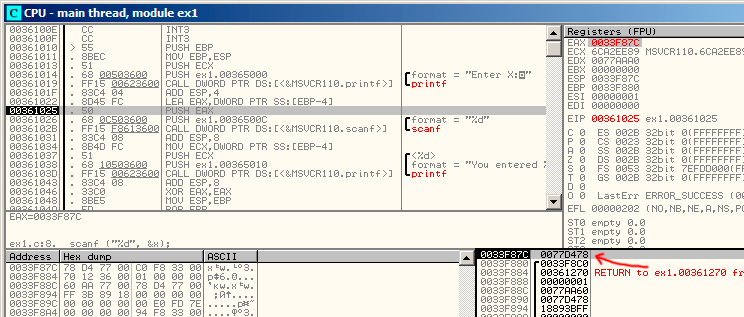
\includegraphics[scale=\FigScale]{patterns/04_scanf/1_simple/ex1_olly_1.png}
\caption{\olly: \RU{вычисляется адрес локальной переменной}\EN{The address of the local variable is calculated}}
\label{fig:scanf_ex1_olly_1}
\end{figure}

\RU{На \EAX в окне регистров можно нажать правой кнопкой и далее выбрать}
\EN{Right-click the \EAX in the registers window and then select} \q{Follow in stack}.
\RU{Этот адрес покажется в окне стека.}
\EN{This address will appear in the stack window.}
\RU{Смотрите, это переменная в локальном стеке. Я нарисовал там красную стрелку}\EN{The red arrow, I have added, points to the variable in the local stack}.
\RU{И там сейчас какой-то мусор}\EN{At that moment this location contains some garbage} (\TT{0x6E494714}).
\RU{Адрес этого элемента стека сейчас, при помощи \PUSH запишется в этот же стек рядом}%
\EN{Now with the help of \PUSH instruction the address of this stack element is going to be stored to the same stack on the next position}.
\RU{Трассируем при помощи F8 вплоть до конца исполнения \scanf}\EN{Let's trace with F8 until the \scanf execution completes}.
\RU{А пока \scanf исполняется, в консольном окне, вводим, например, 123}%
\EN{During the \scanf execution, we input, for example, 123, in the console window}:

\begin{figure}[H]
\centering
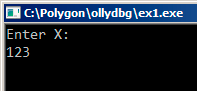
\includegraphics[scale=\NormalScale]{patterns/04_scanf/1_simple/ex1_olly_2.png}
\caption{\RU{Ввод пользователя в консольном окне}\EN{User input in the console window}}
\label{fig:scanf_ex1_olly_2}
\end{figure}

\clearpage
\RU{Вот тут }\scanf \RU{отработал}\EN{completed its execution already}:

\begin{figure}[H]
\centering
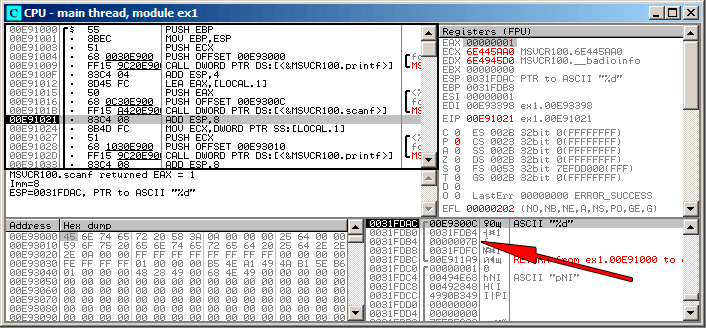
\includegraphics[scale=\FigScale]{patterns/04_scanf/1_simple/ex1_olly_3.png}
\caption{\olly: \scanf \RU{исполнилась}\EN{executed}}
\label{fig:scanf_ex1_olly_3}
\end{figure}

\scanf \RU{вернул}\EN{returns} $1$ \InENRU \EAX, \RU{что означает, что он успешно прочитал одно 
значение}\EN{which implies that it has read successfully one value}.
\RU{В наблюдаемом нами элементе стека теперь}\EN{If we look again at the stack element corresponding to the local variable it now contains} \TT{0x7B} (123).

\clearpage
\RU{Чуть позже это значение копируется из стека в регистр \ECX и передается в \printf}
\EN{Later this value is copied from the stack to the \ECX register and passed to \printf}:

\begin{figure}[H]
\centering
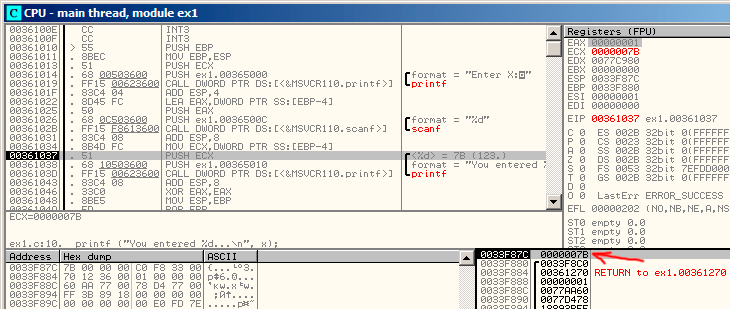
\includegraphics[scale=\FigScale]{patterns/04_scanf/1_simple/ex1_olly_4.png}
\caption{\olly: \RU{готовим значение для передачи в}\EN{preparing the value for passing to} \printf}
\label{fig:scanf_ex1_olly_4}
\end{figure}

\fi

\subsubsection{GCC}

\RU{Попробуем тоже самое скомпилировать в Linux при помощи GCC 4.4.1:}
\EN{Let's try to compile this code in GCC 4.4.1 under Linux:}

\lstinputlisting{patterns/04_scanf/1_simple/ex1_GCC.asm}

\index{puts() \RU{вместо}\EN{instead of} printf()}
\RU{GCC заменил первый вызов \printf на \puts, почему это было сделано, 
уже было описано раннее~(\myref{puts}).}
\EN{GCC replaced the \printf call with call to \puts. The reason for this was explained in ~(\myref{puts}).}

% TODO: rewrite
%\RU{Почему \scanf переименовали в \TT{\_\_\_isoc99\_scanf}, я честно говоря, пока не знаю.}
%\EN{Why \scanf is renamed to \TT{\_\_\_isoc99\_scanf}, I do not know yet.}
% 
% Apparently it has to do with the ISO c99 standard compliance. By default GCC allows specifying a standard to adhere to.
% For example if you compile with -std=c89 the outputted assmebly file will contain scanf and not __isoc99__scanf. I guess current GCC version adhares to c99 by default.
% According to my understanding the two implementations differ in the set of suported modifyers (See printf man page)


\RU{Далее все как и прежде ~--- параметры заталкиваются через стек при помощи \MOV.}
\EN{As in the MSVC example ~---the arguments are placed on the stack using the \MOV instruction.}
\subsection{x64}

\index{x86-64}
\RU{Всё то же самое, только используются регистры вместо стека для передачи аргументов функций.}%
\EN{The picture here is similar with the difference that the registers, rather than the stack, are used for arguments passing.}%
\PTBR{A situação aqui é parecida, mas com a diferença de que os registradores, ao invés da pilha, são usados para passar argumentos.}%

\subsubsection{MSVC}

\lstinputlisting[caption=MSVC 2012 x64]{patterns/04_scanf/1_simple/ex1_MSVC_x64.asm.\LANG}

\ifdefined\IncludeGCC
\subsubsection{GCC}

\lstinputlisting[caption=\Optimizing GCC 4.4.6 x64]{patterns/04_scanf/1_simple/ex1_GCC_x64.s.\LANG}
\fi

\subsection{ARM}

\subsubsection{\OptimizingKeilVI (\ThumbMode)}

\begin{lstlisting}
.text:00000042             scanf_main
.text:00000042
.text:00000042             var_8           = -8
.text:00000042
.text:00000042 08 B5                       PUSH    {R3,LR}
.text:00000044 A9 A0                       ADR     R0, aEnterX     ; "Enter X:\n"
.text:00000046 06 F0 D3 F8                 BL      __2printf
.text:0000004A 69 46                       MOV     R1, SP
.text:0000004C AA A0                       ADR     R0, aD          ; "%d"
.text:0000004E 06 F0 CD F8                 BL      __0scanf
.text:00000052 00 99                       LDR     R1, [SP,#8+var_8]
.text:00000054 A9 A0                       ADR     R0, aYouEnteredD___ ; "You entered %d...\n"
.text:00000056 06 F0 CB F8                 BL      __2printf
.text:0000005A 00 20                       MOVS    R0, #0
.text:0000005C 08 BD                       POP     {R3,PC}
\end{lstlisting}

\index{\CLanguageElements!\Pointers}
\RU{Чтобы \scanf мог вернуть значение, ему нужно передать указатель на переменную типа \Tint.}
\EN{In order for \scanf to be able to read item it needs a parameter---pointer to an \Tint.}
\Tint\RU{~--- 32-битное значение, для его хранения нужно только 4 байта, и оно помещается в 
32-битный регистр.}
\EN{is 32-bit, so we need 4 bytes to store it somewhere in memory, and it fits exactly 
in a 32-bit register.}
\index{IDA!var\_?}
\RU{Место для локальной переменной \TT{x} выделяется в стеке, \IDA наименовала её \IT{var\_8}. 
Впрочем, место для неё выделять не обязательно, т.к. \glslink{stack pointer}{указатель стека} \ac{SP} уже указывает на место, 
свободное для использования.}\EN{A place for the local variable \TT{x} is allocated in the stack and \IDA
has named it \IT{var\_8}. It is not necessary, however, to allocate a such since \ac{SP} (\gls{stack pointer}) is already pointing to that space and it can be used directly.}
\RU{Так что значение указателя \ac{SP} копируется в регистр \Reg{1}, и вместе с format-строкой, 
передается в \scanf.}
\EN{So, \ac{SP}'s value is copied to the \Reg{1} register and, together with the format-string, passed
to \scanf.}
\index{ARM!\Instructions!LDR}
\RU{Позже, при помощи инструкции \TT{LDR}, это значение перемещается из стека в регистр \Reg{1}, 
чтобы быть переданным в \printf.}\EN{Later, with the help of the \TT{LDR} instruction, this value is moved
from the stack to the \Reg{1} register in order to be passed to \printf.}

\subsubsection{ARM64}

\lstinputlisting[caption=\NonOptimizing GCC 4.9.1 ARM64,numbers=left]{patterns/04_scanf/1_simple/ARM64_GCC491_O0.s.\LANG}

\RU{Под стековый фрейм выделяется 32 байта, что больше чем нужно. Вероятно, это связано с выравниваем по границе памяти?}%
\EN{There is 32 bytes are allocated for stack frame, which is bigger than it needed. Perhaps, some memory aligning issue?}
\RU{Самая интересная часть~--- это поиск места под переменную $x$ в стековом фрейме (строка 22).}
\EN{The most interesting part is finding space for the $x$ variable in the stack frame (line 22).}
\RU{Почему 28? Почему-то, компилятор решил расположить эту переменную в конце стекового фрейма, а не в начале.}%
\EN{Why 28? Somehow, compiler decided to place this variable at the end of stack frame instead of beginning.}
\RU{Адрес потом передается в \scanf, которая просто сохраняет значение, введенное пользователем, в памяти
по этому адресу.}
\EN{The address is passed to \scanf, which just stores the user input value in the memory at that address.}
\RU{Это 32-битное значение типа \Tint}\EN{This is 32-bit value of type \Tint}.
\RU{Значение загружается в строке 27 и затем передается в \printf.}
\EN{The value is fetched at line 27 and then passed to \printf.}


\subsection{MIPS}

\RU{Для переменной $x$ выделено место в стеке, и к нему будут производиться обращения как $\$sp+24$.}
\EN{A place in the local stack is allocated for the $x$ variable, and it is to be referred as $\$sp+24$.}
\myindex{MIPS!\Instructions!LW}
\RU{Её адрес передается в \scanf, а значение прочитанное от пользователя загружается используя 
инструкцию LW (\q{Load Word}~--- загрузить слово) и затем оно передается в \printf.}
\EN{Its address is passed to \scanf, and the user input values is loaded using the LW (\q{Load Word}) instruction
and then passed to \printf.}

\lstinputlisting[caption=\Optimizing GCC 4.4.5 (\assemblyOutput)]{patterns/04_scanf/1_simple/MIPS/ex1.O3.s.\LANG}

\RU{IDA показывает разметку стека следующим образом:}
\EN{IDA displays the stack layout as follows:}

\lstinputlisting[caption=\Optimizing GCC 4.4.5 (IDA)]{patterns/04_scanf/1_simple/MIPS/ex1.O3.IDA.lst.\LANG}

% TODO non-optimized version?

